\section{Symulacja HIL}
\label{sec:symulacja-hil}
Trzon symulacji HIL stanowi symulacja rakiety sterowanej FOK 2 w Simulinku 
stworzona przez dra inż. Dariusza Miedzińskiego \cite{Darek-magisterka}.
Została ona następnie przez Zespół rozwinięta. Dodano do niej między innymi 
łatwą możliwość konfiguracji rakiet i przetwarzanie danych. Przez autora pracy
została zaadaptowana do służenia przeprowadzaniu symulacji HIL.

\begin{figure}[htbp]
    \centering
        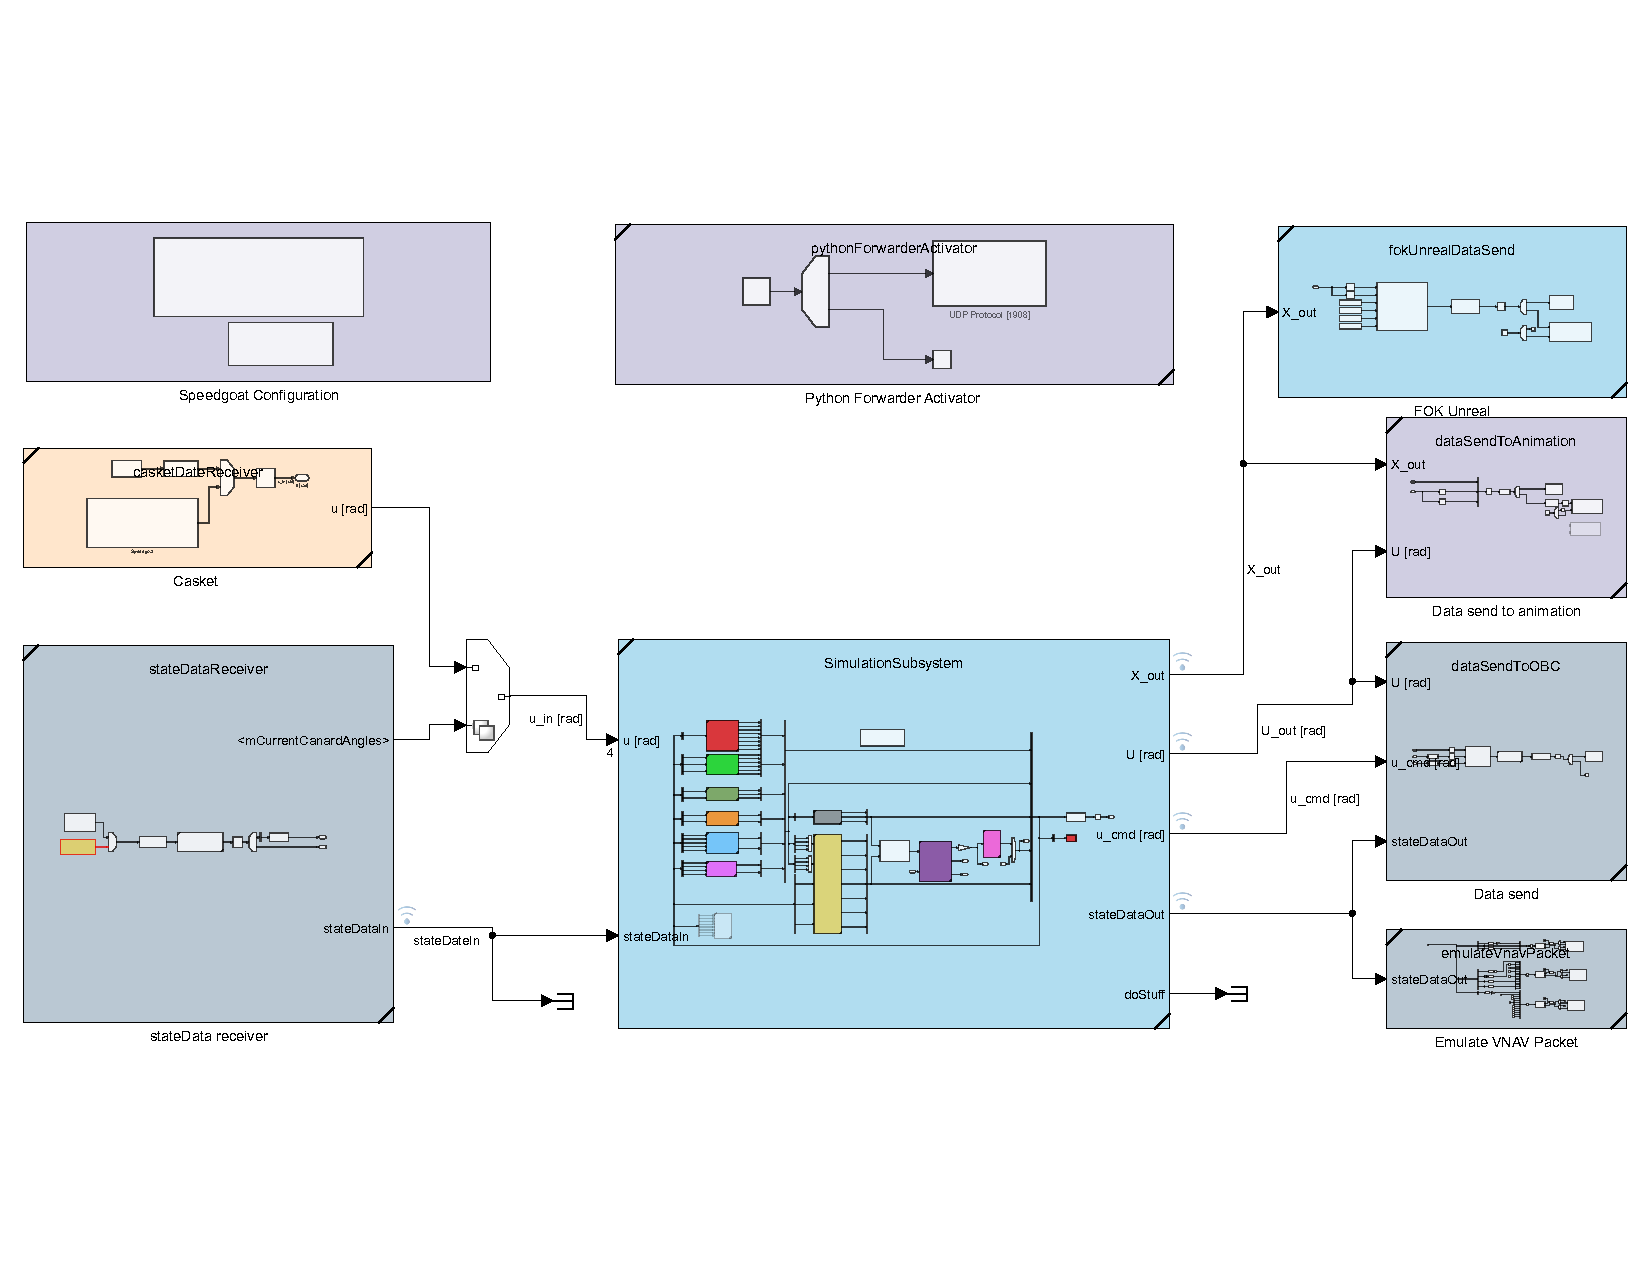
\includegraphics[width=\textwidth,page=1]{Figures/symulacjaSpeedgoatHil.pdf}
    \caption{Widok główny symulacji HIL rakiety FOK 2}
    \label{fig:symulacja-hil-widok-glowny}
\end{figure}

\subsection{Dostosowanie symulacji do badań HIL}
\label{subsec:symulacja-hil-dostosowanie}
Stworzona symulacja HIL jest modułowa. W szczególności każdy z modułów jest
w niej umieszczony za pomocą \textit{Referenced Subsystem}. Pozwala to 
na pracę nad symulacją w wiele osób a także na wielokrotne używanie tych samych
modułów jeżeli jest taka potrzeba. Największym zidentyfikowanym minusem takiego podejścia
jest łatwość, z jaką można w modelu użyć złej wersji danego podsystemu.
Może się tak zdarzyć przykładowo, gdy mamy w ścieżce \textit{MATLAB}a kilka wersji 
symulacji. Dlatego przed właściwą symulacją rekomenduje się restart \textit{MATLAB}a
lub ręczne przejrzenie zawartości ścieżki komendą \texttt{path}.

\subsubsection{Komputer osobisty}
\label{subsubsec:symulacja-hil-dostosowanie-komputer-osobisty}
Przeprowadzanie symulacji HIL na komputerze osobistym z użyciem \textit{Simulink}a
jest wykonywane za pomocą pakietu \textit{Desktop Real-Time} \cite{desktop-realtime}.
Największym problemem w przypadku przeprowadzania symulacji na komputerze osobistym jest trudność
w niezawodnej i pozbawionej opóźnień komunikacji z testowanym urządzeniem. Pakiet \textit{Desktop Real-Time}
nie udostępnia wielu możliwości komunikacji. Spośród dostępnych zdecydowano się wybrać \textit{UDP protocol}.
Jest to zestaw bloczków umożliwiający komunikację w protokole UDP. Zaletą tego wyboru
jest łatwość użycia - obok TCP jest to jeden z dwóch głównych protokołow warstwy transportowej infrastruktury sieciowej.
Jest więc bez żadnych modyfikacji obsługiwany przez każdy komputer osobisty i wiele mikrokontrolerów.
W praktyce, do jego użycia wystarczy jedynie podpiąć komputer przewodem ethernet lub bezprzewodowo 
do routera lub innego urządzenia.

Jednak nawet takie rozwiązanie nie jest pozbawione problemów. 
Pierwszym potencjalnym problemem jest brak gwarancji dostarczenia pakietu danych. W praktyce jednak 
współczesne rozwiązania sieciowe są na tyle niezawodne a użyta infrastruktura testowana na tyle prosta
pod tym względem, że ten problem nie występuje. 
Większym problemem jest brak kontroli nad kolejką pakietów przychodzących do symulacji.
Jako, że moduły systemu testowego mają być z założenia niezależne od siebie, to CASKET i komputer pokładowy 
zaczynają nadawać pakiety niezależnie od momentu rozpoczęcia symulacji. Zdiagnozowano,
że takie zachowanie powoduje nabudowanie kolejki pakietów po stronie odbiorczej symulacji.
Nie znaleziono prostego sposobu by czytać jedynie najnowszy pakiet z poziomu \textit{Simulink}a.
Stworzono więc obejście problemu. Urządzenia nie wysyłają pakietów bezpośrednio do symulacji, a do skryptu pythonowego.
Zadaniem tego skryptu jest następnie przesłanie najnowszego pakietu do symulacji gdy symulacja zostanie uruchomiona.
Zasada działania skryptu jest następująca:
\begin{enumerate}
    \item Oczekiwanie na pakiet aktywacyjny od symulacji.
    \item Odebranie pakietu aktywacyjnego.
    \item Przekazywanie w pętli najnowszych pakietów do symulacji.
\end{enumerate}
Aktywator skryptu pythonowego polega na wysłaniu niepustego pakietu na odpowiedni port.
Widoczny jest on na Rysunku~\ref{fig:symulacja-hil-dostosowanie-komputer-osobisty-przekierowanie}

\begin{figure}[htbp]
    \centering
        \includegraphics[width=0.8\textwidth,page=47, clip,trim={7cm, 7cm, 7cm, 7cm}]{Figures/symulacjaSpeedgoatHil.pdf}
    \caption{Moduł odpowiedzialny za aktywowanie skryptu przekierowującego pakiety do symulacji}
    \label{fig:symulacja-hil-dostosowanie-komputer-osobisty-przekierowanie}
\end{figure}

Takie rozwiązanie może potencjalnie zwiększać opóźnienia i zmniejszać deterministyczność komunikacji.
W toku przeprowadzania testów nie zauważono jednak problemów wynikających z takiego przesyłania pakietów.

Warto nadmienić, że w toku projektu podjęto próbę unifikacji działania \textit{CASKET}a
w przypadku przeprowadzania symulacji na komputerze osobistym i czasu rzeczywistego.
Użycie protokołu SPI do komunikacji z komputerem osobistym wymaga jednak użycia konwertera sygnału.
Nie udało się znaleźć rozwiązania, które byłoby zarówno proste w konfiguracji, użyciu i działałoby z \textit{Simulink}iem.

\todo[inline]{Tutorial przeprowadzenia symulacji}

\subsubsection{Komputer czasu rzeczywistego}
\label{subsubsec:symulacja-hil-dostosowanie-komputer-czasu-rzeczywistego}
Mimo, że przeprowadzanie symulacji HIL jest możliwe na komputerze rzeczywistym to wiąże się to 
z pewnymi ograniczeniami. W szczególności trudnościami z obsługą interfejsów 
oraz zagwarantowaniem czasu rzeczywistego. Oba aspekty są szczególnie ważne gdy
wynik symulacji zależy na komunikacji z innymi urządzeniami.

Przy komunikacji z \textit{CASKET}em użycie go pozwoliło na bezpośrednie podpięcie 
mikrokontrolera obsługującego stanowisko pomiarowe do komputera czasu rzeczywistego używając protokołu SPI.

Drugim aspektem wykorzystania komputera czasu rzeczywistego do symulacji HIL jest 
wykorzystanie go do emulacji pakietów czujnika pokładowego rakiety - VectorNav 200 \cite{vectornav_vn200}.
W obecnej konfiguracji czujnik wysyła komputerowi pokładowemu 3 różne pakiety danych o 
częstotliwość odpowiednio \SI{800}{\hertz}, \SI{400}{\hertz} i \SI{200}{\hertz}:
\begin{enumerate}
    \item przyspieszenie liniowe, prędkość kątowa,
    \item dane z INS, parametry całkowania INS,
    \item dane o niepewnościach, ciśnienie, odczyt magnetometru status czujników.
\end{enumerate}
Ponadto każdy z pakietów zawiera timestamp.
Jako, że interfejsem używanym w rakiecie do komunikacji OBC-czujnik jest UART (TTL), 
to możliwe jest bezpośrednia komunikacja \textit{Speedgoat} - OBC, w której to \textit{Speedgoat}
emuluje czujnik. Teoretycznie z użyciem konwertera powinno być możliwe zaimplementowanie 
tej funkcjonalności w symulacji z komputerem osobistym jednak ta konfiguracja nie była dotąd rozwijana.
Zaimplementowano jedynie komunikację jednostronną - \textit{Speedgoat} emuluje już skonfigurowany
czujnik bez możliwości rekonfiguracji przez komputer pokładowy jak ma to miejsce w przypadku konfiguracji lotnej.
Takie rozwiązanie sprawia że z minimalnymi zmianami w konfiguracji komputera pokładowego 
możliwe jest przeprowadzenie symulacji, podczas której \textit{sądzi on} że odbywa test lotny.
Umożliwia to lepsze odwzorowanie działania komputera podczas lotu przez zapewnienie
identycznych interfejsów a co za tym idzie interakcji między różnymi komponentami rakiety, 
czasami odczytu danych co w przypadku prawdziwego lotu.

\begin{figure}[htbp]
    \centering
        \missingfigure{Schemat komunikacji ze speedgoatem}
    \caption{Schemat konfiguracji CASKET-Speedgoat}
    \label{fig:symulacja-hil-dostosowanie-komputer-czasu-rzeczywistego-schemat-speedgoat}
\end{figure}

\todo[inline]{Tutorial przeprowadzenia symulacji}